% Created 2020-10-06 Tue 18:02
% Intended LaTeX compiler: pdflatex
\documentclass[11pt]{article}
\usepackage[utf8]{inputenc}
\usepackage[T1]{fontenc}
\usepackage{graphicx}
\usepackage{grffile}
\usepackage{longtable}
\usepackage{wrapfig}
\usepackage{rotating}
\usepackage[normalem]{ulem}
\usepackage{amsmath}
\usepackage{textcomp}
\usepackage{amssymb}
\usepackage{capt-of}
\usepackage{hyperref}
\usepackage{graphicx}
\usepackage{dsfont}
\author{Oscar Morris}
\date{}
\title{Continuous Fractions}
\hypersetup{
 pdfauthor={Oscar Morris},
 pdftitle={Continuous Fractions},
 pdfkeywords={},
 pdfsubject={},
 pdfcreator={Emacs 27.1 (Org mode 9.4)}, 
 pdflang={English}}
\begin{document}

\maketitle
\tableofcontents


\section{Introduction}
\label{sec:orgd1732b9}
The continuous fraction \(1+\frac{1}{1+\frac{1}{\dots}}\) which can be generalised as \(t_n=k+\frac{1}{t_{n-1}}\) where \(k \in \mathds{R}\). When the first 15 terms \(t_n\) where \(k=1\) are plotted \(t_n\) against \(n\) you get the following chart:
\begin{figure}[h]
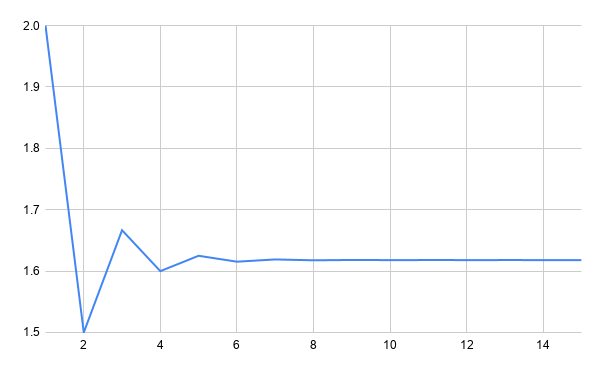
\includegraphics[scale=0.5]{chart1}
\end{figure}
Using the graph the observation can be made that the value of \(t_n\) converges on a specific value \(\approx 1.618033988749895\) therefore it can be determined that \(t_{n-1}-t_n\) approaches \(0\). The problems arisisng for high values of \(n\) is that you quickly reach the limit of floating point maths used by computers.
\section{Differing values of k}
\label{sec:org7584de5}
\subsection{\(k=2\)}
\label{sec:org1b5715e}
The graph of the generalised equation \(t_n=k+\frac{1}{t_{n-1}}\) where \(k=2\) is below:
\begin{figure}[h]
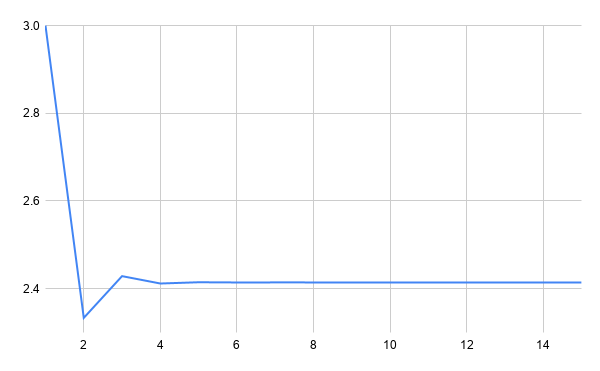
\includegraphics[scale=0.5]{chart2}
\end{figure}
From this graph a similar observation can be made as the case where \(k=1\) being that the value of \(t_n\) converges on a specific value \(\approx 2.4142135623731\) however is seems to converge to this value more quickly.
\subsection{\(k=0\)}
\label{sec:org53b53f8}
When \(k=0\) the value of \(t_n\) stays constant at \(1\) which would be expected since having a non-zero value of \(k\) is what allows the value of \(t_n\) to converge    .
\subsection{\(k < -1\)}
\label{sec:org43b7c5c}
Here since the value of \(k\) is given as an uncertainty we can take \(k=-1\) and \(k=-2\) and extrapolate from there. There is only a value for \(t_n\) where \(n=1\) since the value of \(t_1=1-1=0\) therefore every value of \(t_n\) for higher values of \(n\) will be a division by \(0\).
For \(k=-2\), the graph displays characteristics to both the graph where \(k=1\) and where \(k=2\) and is shown below:
Here the graph appears similar the the graph of \(k=2\) however it's starting value is -1. It converges on a value \(\approx -2.4142135623731\) which is the negative of the value that \(k=2\) converges on
\subsection{\(0 < k < -1\)}
\label{sec:org2181fcc}
Some of the graphs of values of \(k\) between 0 and -1 are somewhat unusual however the graph of \(k=0.5\) is below:
This graph is mostly expected as it converges slower than when \(k=1\) however the spike at \(n=4\) is mostly unexpected, the value of \(t_4=5.5\).
The graph where \(k=-0.1\) is the most unexpected however \(t_n\) seems to diverge as \(n\) increases, the graph is below:
\section{Determining exact limits}
\label{sec:org1ca692f}
Since some of these continued fractions converge there must be an exact value for \(t_{\infty}\) which we can calculate. Using the continued fraction \(1+\frac{1}{1+\frac{1}{\dots}}\) the limit is as follows:
Consider the quadratic \(x^2-x-1=0\), to find it's solutions we can use the quadratic formula:
\begin{equation*}
x=\frac{-b \pm \sqrt{b^2 - 4ac}}{2a}
\end{equation*}
Solving for \(x\) where \(a=1\), \(b=-1\), \(c=-1\) we get the solutions \(x=\frac{1+\sqrt{5}}{2}\) (the positive solution) or \(x=\frac{1-\sqrt{5}}{2}\) (the negative solution). If we consider the positive value of \(x\) as \(\Phi\) we can say that:
\begin{equation*}
\Phi^2-\Phi-1=0
\end{equation*}
Rearranging this equation we get:
\begin{equation*}
\Phi=1+\frac{1}{\Phi}
\end{equation*}
If we substitute \(\Phi\) into the right side we get:
\begin{equation*}
\Phi=1+\frac{1}{1+\frac{1}{\Phi}}
\end{equation*}
If we repeat this substitution ``to infinity'' we get the continued fraction above.
This indicates that the exact value for this continued fraction is \(\frac{1+\sqrt{5}}{2}\) which bears a fairly high amount of significance as it equals the \textbf{golden ratio} which is often given the capital letter phi (\(\Phi\))
\end{document}
